\chapter{evaluation}\label{chapter:evaluation}

To evaluate the project researchers at both Imperial College London and Kings College London have been consulted for feedback. Since the evaluation group is relatively small (9 users), the interviews were focused on gaining personal insights, rather than trying to amass data that, due to the sample size, no statistical conclusions could be drawn from.

The feedback sessions took the form of a structured interview where features were demonstrated, discussed and then some more traditional questionnaire questions were asked. I found that the most useful feedback came from informally speaking to the researchers as it gave a more personal glimpse into their world than a questionnaire ever could. 

\section{Scan Simulation}
The feedback required for scan simulation was firstly to determine whether or not this would be a useful tool for the researchers. If it was, then the limitations of the current implementation needed to be found to guide the development. In particular are all the parameters usually present when setting up an MRI scan available and what other artefacts are there that would be useful to simulate?

The researchers were asked 'How useful is this feature for you?' and their responses are shown below in figure \ref{fig:graph_scansimulation_1}.

\begin{figure}[h]
    \centering
	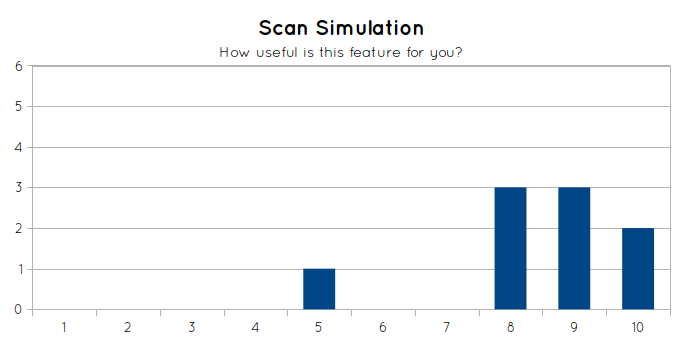
\includegraphics[width=0.6\textwidth]{images/evaluation/graph_scan_simulation_1.png}
    \caption{1 is useless. 10 is very useful.}\label{fig:graph_scansimulation_1}
\end{figure}

The majority of users thought that this feature would be of use for them. The one notable exception on the graph was due to concerns that the complexity of the simulation currently implemented is a far cry from that required. More on that shortly.

The users were then asked 'Does it include all of the parameters that you would expect?' and 'Is the simulation realistic enough?' to get an idea of what other features need to be implemented. Their responses are shown in figure \ref{fig:graph_scan_simulation23}.

\begin{figure}[H]
  \centering
  \begin{subfigure}[b]{0.5\textwidth}
    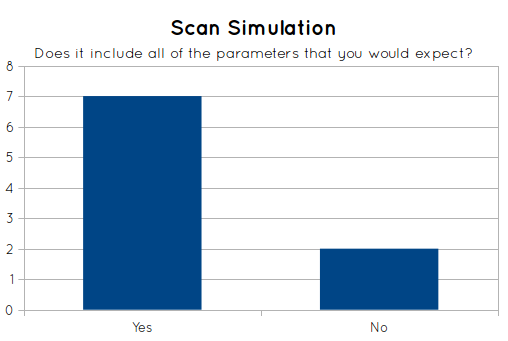
\includegraphics[width=\textwidth]{images/evaluation/graph_scan_simulation_2.png}
    %\caption{Variation 1}
    %\label{fig:graph_scansimulation_2}
  \end{subfigure}%
  ~ %add desired spacing between images, e. g. ~, \quad, \qquad, \hfill etc.
    %(or a blank line to force the subfigure onto a new line)
  \begin{subfigure}[b]{0.5\textwidth}
    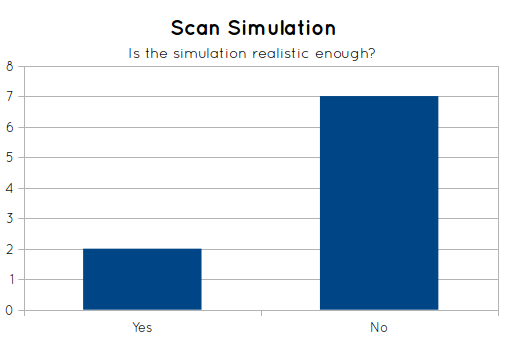
\includegraphics[width=\textwidth]{images/evaluation/graph_scan_simulation_3.png}
    %\caption{Variation 2}
    %\label{fig:graph_scansimulation_3}
  \end{subfigure}
  \caption{Responses to realism questions.}\label{fig:graph_scan_simulation23}
\end{figure}

For the most part the researchers felt that the control they have over the scan configuration was enough. One suggested that instead of specifying the value in pixels, which was a natural unit to use when dealing with a reconstructed volume, it would be good to have the option to specify mm instead, which more closely matches a MRI scanner. 

Another suggestion was the ability to specify a scan by selecting the two endpoints. This would give the user finer directional control and the ability to more easily specify shorter scans.

The question about the realism required of the simulation prompted the largest response. Quickly the feature list for potential improvements grew. As a reminder the only artefact currently implemented is a simple rotation which takes effect in between scanning slices.

\begin{itemize}
  \item \textbf{Additional movement artefacts.} Movement during an MRI scan does not manifest itself as blur, like many other imaging techniques. Instead a number of different artefacts occur including replication, where multiple copies of the object appear, or shadowing where objects in motion appears darker than their surroundings.

  \item \textbf{Translation + Enhanced Rotation}. Translations can be added alongside the rotations but there are also more fundamental changes that can be made to model the movement more realistically. Currently a uniform random variable decides the random rotation and this is unlikely to match the genuine movement of a fetus. For example a fetus is far more likely to nod than shake it's head. Data on fetal movement has been collected at different stages of development previously to establish behavioural patterns\cite{fetalmovement} and so this data could be repurposed to sample movements from a more representative distribution.

  \item \textbf{Interleaved acquisition.} Currently neighbouring slices in the simulated scan are acquired sequentially however in reality the order the slices are acquired is often interleaved (e.g. 1, 5, 10, ..., 2, 6, 11, ...). This is because the frequency of radio wave used to acquire a single slice isn't perfect and so when one slice is excited, slices adjacent to it are often excited as well, albeit to a lesser extent\cite{basicsofmri}. Scanning in an interleaved manner allows these adjacent slices time to relax before they are acquired. The upshot of this is that neighbouring slices are likely to be acquired further apart in time than those in the interleaved set. When simulating movement this sequence can be taken into account.

  \item \textbf{Bias/Inhomogeneity.} The proximity of the fetus from the receiver coil can also have an effect on the scan. This can often create what is known as a bias or inhomogeneity which effectively results in areas of the scan being darker than they should be.

  \item \textbf{Noise.} The signal to noise ratio (SNR) plays an important role in deciding what resolution to scan at. Too high and the image will be too noisy, but too low and the image will be too blurry. Interestingly the noise that appears in MRI scans is not Gaussian, but Rician. This is because the image is acquired in the frequency domain (known as k-space) and this information is transformed to build an image space representation. Since the noise is Gaussian in the frequency domain it becomes Rician in the spatial domain.
  
  \item \textbf{Extend to Moving/Periodic Scans.} The way that a cine (moving MRI image) is acquired differs from the imaging of a static object. For periodic motion, like the beating of the heart, a number of scans are acquired and then those that happen to be at the same point in the cycle are used to reconstruct one frame in the animation. This is another area that could potentially be simulated.
\end{itemize}

\newpage
\section{Reconstruction}
The purpose of this part of the plugin was to get an idea of how researchers feel about manually labelling slice stacks to improve the quality of the reconstruction. 

When asked 'How important is it for you to manually guide the reconstruction process?' the majority preferred to have some degree of control over it. See figure \ref{fig:graph_reconstruction_1}. Those who were less concerned about this either weren't involved in the reconstruction process (and put 1) or felt that they do like the ability to guide it but would greatly prefer if it were automated.

\begin{figure}[h]
    \centering
  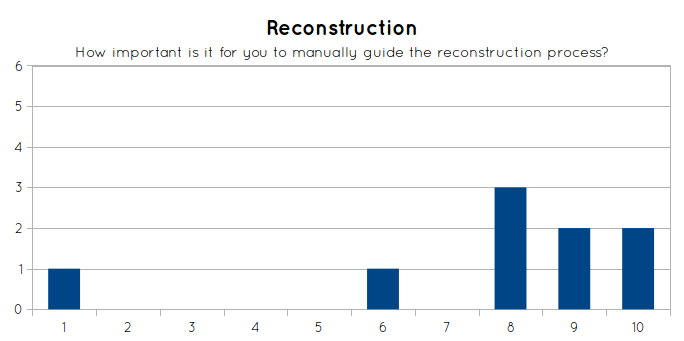
\includegraphics[width=0.6\textwidth]{images/evaluation/graph_reconstruction_1.png}
    \caption{1 is not at all. 10 is very important.}\label{fig:graph_reconstruction_1}
\end{figure}

When asked 'How likely are you to manually label stack sets to improve the reconstruction?' the responses were more varied. See figure \ref{fig:graph_reconstruction_2}. Most participants were willing to label slice stacks but there was more negativity towards this than before, and the impression received was that they do it begrudgingly.

Anecdotally it seems to take around 30 minutes to perform the pre-processing required for a single reconstruction. This involves manually inspecting each slice to gauge the quality, building a mask to specify the area to reconstruct and optionally adding landmarks to each stack.

Currently four landmarks can be used to aid the registration: both eyes and two points on the brain stem. In some cases, where the input data is good, this is not necessary, however if there is a large amount of movement then manual intervention is required.

When asked 'How long would you be willing to spend labelling landmarks for a reconstruction?' nobody was willing to spend more than 30 minutes and the majority would prefer it to take 10 minutes or below. See figure \ref{fig:graph_reconstruction_3}. It's difficult to say whether there may be some degree of "asking for more than you expect to get" going on but the consensus is that the time quickly adds up. It's fine if you have one reconstruction to do but when you come to large user studies with potentially hundreds of scans it simply doesn't scale.

\begin{figure}[H]
  \centering
  \begin{subfigure}[b]{0.5\textwidth}
    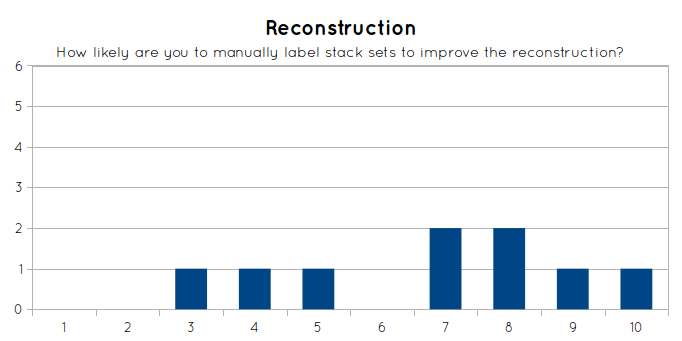
\includegraphics[width=\textwidth]{images/evaluation/graph_reconstruction_2.png}
    \caption{1 is no chance, 10 is very likely.}
    \label{fig:graph_reconstruction_2}
  \end{subfigure}%
  ~ %add desired spacing between images, e. g. ~, \quad, \qquad, \hfill etc.
    %(or a blank line to force the subfigure onto a new line)
  \begin{subfigure}[b]{0.5\textwidth}
    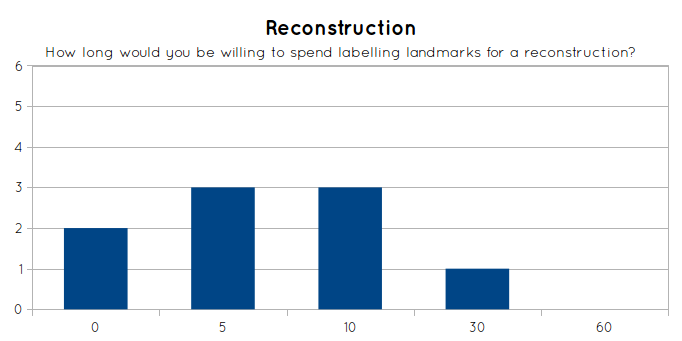
\includegraphics[width=\textwidth]{images/evaluation/graph_reconstruction_3.png}
    \caption{Time (minutes).}
    \label{fig:graph_reconstruction_3}
  \end{subfigure}
  \caption{}\label{fig:graph_reconstruction23}
\end{figure}

The plugin includes a simple tool that allows 13 landmarks to be specified on each slice stack before reconstruction. This was implemented with the view of trying to estimate how long the landmarking stage takes to perform. Constraints on how long I had to spend with each user on the evaluation, and also the level of familiarity of each user with the developing brain mean that the estimations here are quite rough, but do set the scene.

5 users were familiar enough with the brain to take part in the time trial. The stacks being annotated had been simulated with up to 5 degrees of motion corruption but other than that was very clean and so there is little ambiguity finding the points. The times are shown in figure \ref{fig:landmarktimes}.

\begin{figure}[h]
    \centering
  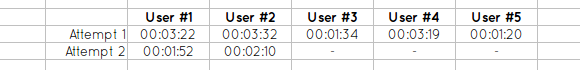
\includegraphics[width=0.8\textwidth]{images/evaluation/graph_reconstruction_landmark_times.png}
    \caption{There is large variance, but around 2 minutes seems reasonable.}\label{fig:landmarktimes}
\end{figure}

Taking these results with a pinch of salt it seems that around 10 seconds per landmark is a reasonable estimate, once the user is up to speed. With a large number of stacks per reconstruction and a large number of reconstructions in a study this soon adds up.

Another source of inefficiency comes from the use of a number of different pieces of software in the reconstruction process. Integrating the process into one application should remove the time wasted importing and exporting between different tools.

One problem that had not been anticipated were ambiguities determining which direction is left and which is right when placing landmarks. This is one of the limitations of DICOM, one of the most common medical image formats in use, and so some way of letting the user mark this, before a mask is created, would be useful.

The researchers still want a way to manually inspect the slice stacks to check their quality, either to establish why a reconstruction failed, or as a preliminary check. One feature that could be implemented to help with this is the ability to view stacks side by side and scroll through them simultaneously.

Another issue raised was that there was ambiguity deciding which part of a landmark to mark. Having an example image for each would clarify both what the user is looking for and also where to mark it.

\newpage
\section{Visualizations - Uncertainty}
There are three things that make a good visualization. Firstly you must be able to understand what it is showing; a visualization can look fantastic but if you can't understand what you're looking at then it is useless. Secondly it must be clear; an uncertainty visualization should communicate the uncertainty without unnecessary complication which will distract the viewer from what is important. Thirdly it must be configurable; being able to tweak a visualization to highlight different areas of interest makes it more flexible and useful in a wider range of scenarios.

With these three principles in mind the users were asked three questions for each visualization. The first they were asked was 'How easy was it to understand what the visualization was showing?'. The results for each visualization are shown in figure \ref{fig:eval_visualization_q1}.

\begin{figure}[H]
  \centering
  \begin{subfigure}[b]{0.5\textwidth}
    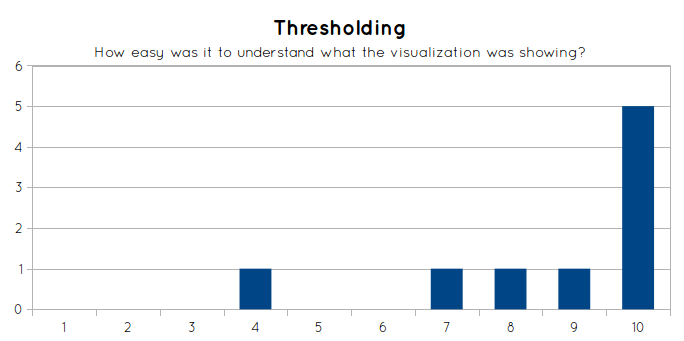
\includegraphics[width=\textwidth]{images/evaluation/graph_thresholding_1.png}
    \caption*{Thresholding}
    \label{fig:eval_visualization_q1_thresholding}
  \end{subfigure}%
  ~ %add desired spacing between images, e. g. ~, \quad, \qquad, \hfill etc.
    %(or a blank line to force the subfigure onto a new line)
  \begin{subfigure}[b]{0.5\textwidth}
    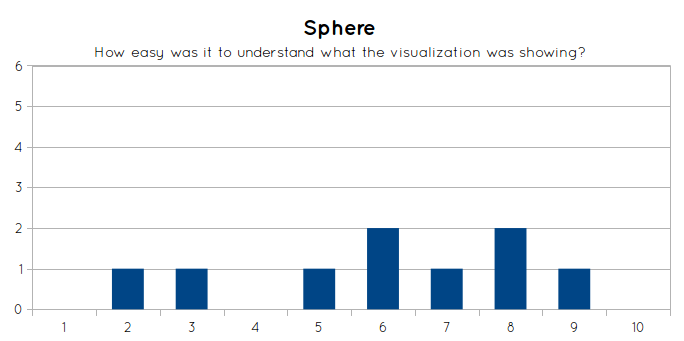
\includegraphics[width=\textwidth]{images/evaluation/graph_sphere_1.png}
    \caption*{Sphere}
    \label{fig:eval_visualization_q1_sphere}
  \end{subfigure}
  ~ %add desired spacing between images, e. g. ~, \quad, \qquad, \hfill etc.
    %(or a blank line to force the subfigure onto a new line)
  \begin{subfigure}[b]{0.5\textwidth}
    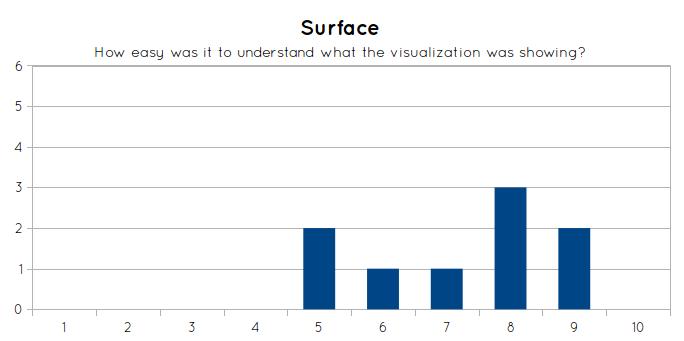
\includegraphics[width=\textwidth]{images/evaluation/graph_surface_1.png}
    \caption*{Surface}
    \label{fig:eval_visualization_q1_surface}  
  \end{subfigure}
  \caption{1 is very difficult. 10 is very easy.}\label{fig:eval_visualization_q1}
\end{figure}

The easiest visualization to understand overall was thresholding. From speaking to the researchers this was because they are very familiar with this kind of view, especially the 2D version; a lot of their work involves them examining slice stacks and scrolling through data sets.

Conceptually it is also the easiest visualization to grasp, the uncertainty is simply overlayed on the scan in 2D and you can see it floating around in 3D. For them to use the surface view there needs to be a compelling, unique feature that can't be done with thresholding.

The sphere was the hardest to understand with some users ranking it as low as 2 or 3 out of 10. The biggest problem people had with the sphere was the lack of a grounding and this sense of disjointness with the raw data put many people off.

Whilst not as easy to understand as thresholding, the surface (built from the reconstruction mask) was better received than the sphere. The surface fixes the main issue that the sphere has by giving a sense of where in the scan you are looking at, which the users seemed to like. However currently the surface used to represent the brain is still fairly rough, and whilst it does resemble a brain it isn't as clear as perhaps it could be.

The second question they were asked was 'How clearly did the visualization highlight the most uncertain region?'. The results are shown in figure \ref{fig:eval_visualization_q2}.

\begin{figure}[H]
  \centering
  \begin{subfigure}[b]{0.5\textwidth}
    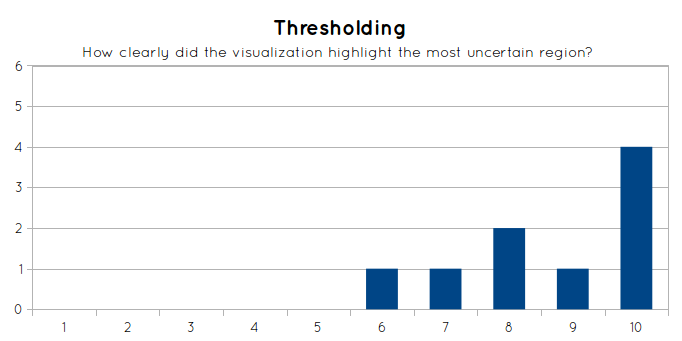
\includegraphics[width=\textwidth]{images/evaluation/graph_thresholding_2.png}
    \caption*{Thresholding}
    \label{fig:eval_visualization_q2_thresholding}
  \end{subfigure}%
  ~ %add desired spacing between images, e. g. ~, \quad, \qquad, \hfill etc.
    %(or a blank line to force the subfigure onto a new line)
  \begin{subfigure}[b]{0.5\textwidth}
    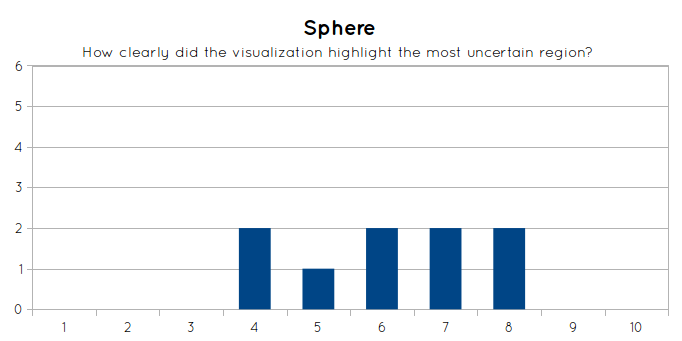
\includegraphics[width=\textwidth]{images/evaluation/graph_sphere_2.png}
    \caption*{Sphere}
    \label{fig:eval_visualization_q2_sphere}
  \end{subfigure}
  ~ %add desired spacing between images, e. g. ~, \quad, \qquad, \hfill etc.
    %(or a blank line to force the subfigure onto a new line)
  \begin{subfigure}[b]{0.5\textwidth}
    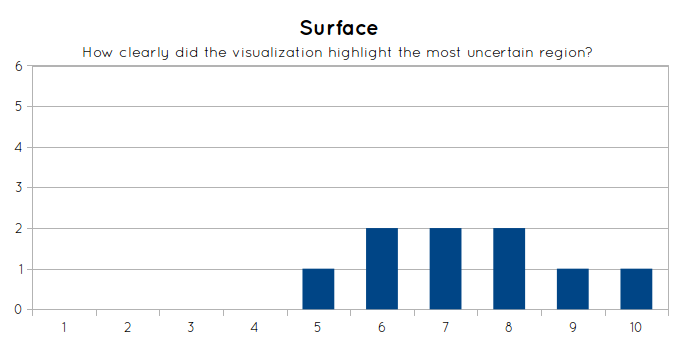
\includegraphics[width=\textwidth]{images/evaluation/graph_surface_2.png}
    \caption*{Surface}
    \label{fig:eval_visualization_q2_surface}  
  \end{subfigure}
  \caption{1 is not at all clear. 10 is very clear.}\label{fig:eval_visualization_q2}
\end{figure}

The results show a similar story to the first question. Thresholding was deemed the clearest at highlighting areas of high uncertainty. Speaking to the researchers suggests that this was because with thresholding the exact location of the uncertainty could be determined, whereas the other visualizations only narrowed it down to a region.

The surface visualization was the next best, followed by the sphere. Feedback suggests that it was easier to understand where the uncertainty was in the surface because there was a point of reference which simply was not present in the sphere.

The users were then asked 'How easy was the visualization to configure to target different areas of interest?'. The results are shown in figure \ref{fig:eval_visualization_q3}.

\begin{figure}[H]
  \centering
  \begin{subfigure}[b]{0.5\textwidth}
    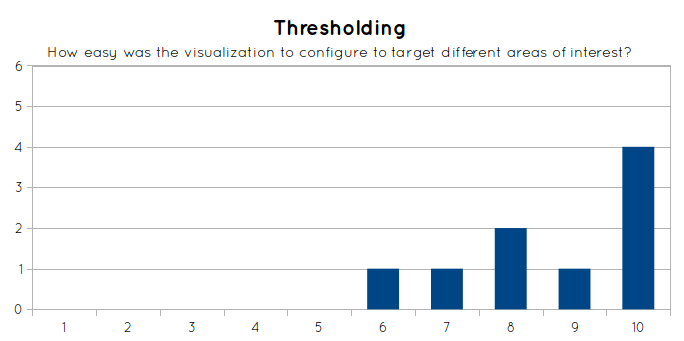
\includegraphics[width=\textwidth]{images/evaluation/graph_thresholding_3.png}
    \caption*{Thresholding}
    \label{fig:eval_visualization_q3_thresholding}
  \end{subfigure}%
  ~ %add desired spacing between images, e. g. ~, \quad, \qquad, \hfill etc.
    %(or a blank line to force the subfigure onto a new line)
  \begin{subfigure}[b]{0.5\textwidth}
    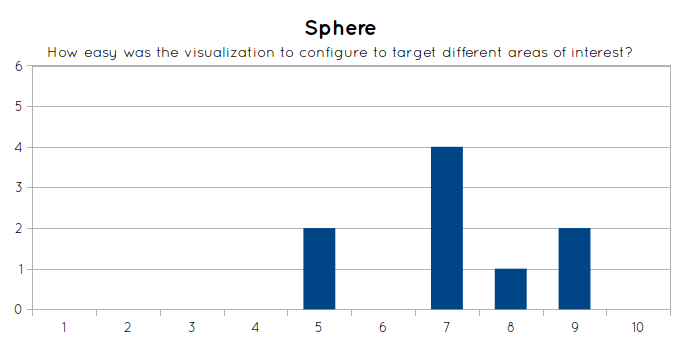
\includegraphics[width=\textwidth]{images/evaluation/graph_sphere_3.png}
    \caption*{Sphere}
    \label{fig:eval_visualization_q3_sphere}
  \end{subfigure}
  ~ %add desired spacing between images, e. g. ~, \quad, \qquad, \hfill etc.
    %(or a blank line to force the subfigure onto a new line)
  \begin{subfigure}[b]{0.5\textwidth}
    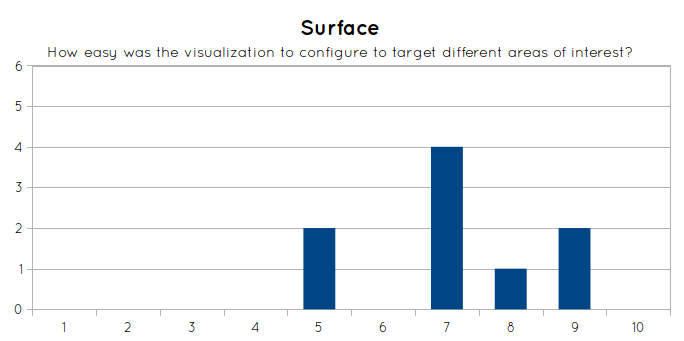
\includegraphics[width=\textwidth]{images/evaluation/graph_surface_3.png}
    \caption*{Surface}
    \label{fig:eval_visualization_q3_surface}  
  \end{subfigure}
  \caption{1 is very difficult. 10 is very easy.}\label{fig:eval_visualization_q3}
\end{figure}

Again the thresholding was deemed easiest to control, at least in part due to the simplicity of the options available: you either define a range of uncertainty to see or view the worst $x\%$. Interestingly the surface and sphere swapped roles and the sphere was deemed easier to control than the surface.

Largely they have the same controls; both allow you to specify how far into the volume to sample (half/full) and how to accumulate uncertainty (average/worst/best). However, the surface visualization adds the complication of picking the right combination of surface model and registration options to get it to function correctly. Clearly these options need to be better documented or presented differently to avoid confusion.

A common insight for each of the visualizations was that it would be useful to have the ability to target specific areas of the brain to show just the uncertainty in that region. Often researchers only care about one area; for example they may be interested in computing the volume of a certain region. This could be achieved relatively simply by allowing the user to create a custom mask or by having a set of general masks that can be registered to the reconstruction.

\newpage
\section{Visualizations - Next Scan Plane}
The same three principles used to evaluate the uncertainty visualizations apply to visualizing the next scan plane. The only difference is that the information being communicated is focused on a scan, not the uncertainty.

The researchers were initially asked 'How easy was it to understand what the visualization was showing?'. The responses are shown in figure \ref{fig:eval_next_scan_plane_q1}.

\begin{figure}[h]
    \centering
  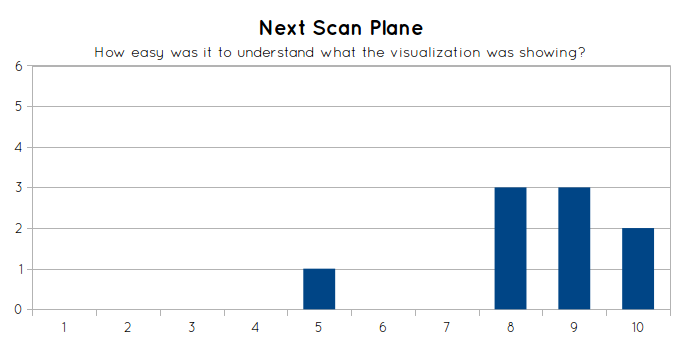
\includegraphics[width=0.6\textwidth]{images/evaluation/graph_next_scan_plane_1.png}
    \caption{1 is very difficult. 10 is very easy.}\label{fig:eval_next_scan_plane_q1}
\end{figure}

Generally it seems the visualization is easy to understand. It was mentioned that using a cylinder to represent the scanning direction is slightly ambiguous as it was unclear which direction it was intended to represent. In fact the direction could be either way and so the ambiguity is intended but to make it clear that it is representing a direction an arrow would be more explicit.

The next question asked was 'How clearly did the visualization illustrate the next best scan plane?'. The responses are shown in figure \ref{fig:eval_next_scan_plane_q2}.

\begin{figure}[h]
    \centering
  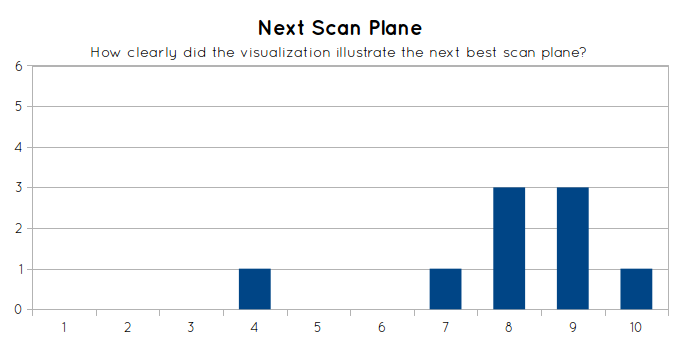
\includegraphics[width=0.6\textwidth]{images/evaluation/graph_next_scan_plane_2.png}
    \caption{1 is not at all clear. 10 is very clear.}\label{fig:eval_next_scan_plane_q2}
\end{figure}

Most users felt that the visualization was clear, although similarly to the sphere visualization some found it to be a little detached from the scan, especially in 3D. Adding some axes to refer to would give some context to the directions. Another point raised was that on the MRI scanner used by one of the researchers the scan direction was not specified by a vector, but by angles. Adapting the format, or adding the option to display it like this would be a very simple change.

Then they were asked 'How easy was the visualization to configure to target different areas of interest?'. The responses are shown in figure \ref{fig:eval_next_scan_plane_q3}.

\begin{figure}[h]
    \centering
  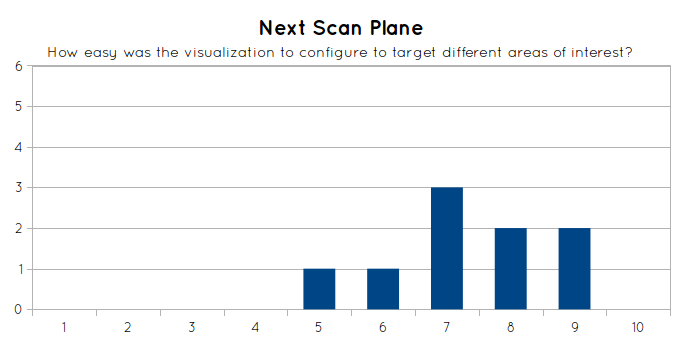
\includegraphics[width=0.6\textwidth]{images/evaluation/graph_next_scan_plane_3.png}
    \caption{1 is very difficult. 10 is very easy.}\label{fig:eval_next_scan_plane_q3}
\end{figure}

Again the results are largely positive with most liking the ability to target values that were particularly bad, however more control would be preferred. In particular it would be useful to be able to target specific regions of the brain; for example if they are only interested in the prefrontal cortex it would be beneficial to specifically target, or give more importance to, uncertain points in that region.

Those researchers who were involved with actually performing scans were asked if the visualization was necessary or whether they would be happy for the scanner to automatically set up the next scan without showing it to them. The response was resoundingly in favour of the visualization; having control of the scan is very important for them as it allows them to take into account factors, such as particular scanner limitations, that the technique may not know about.

An additional benefit of this visualization is that it would allow the radiographer to isolate smaller areas that needed further scanning. Instead of acquiring a complete stack which may take 3 minutes, this allows them to focus on a smaller region which could be acquired in less time and only generate data that was genuinely needed. This tightens up the feedback loop allowing more smaller scans to be taken to target problem areas.